\subsection{Løsningsstrategi}
Vi vil i vores projekt tage en anden tilgang til problemløsningen end de andre software-produkter, vi undersøgte i afsnit \ref{sota}. Vi vil i stedet gøre som naturen gør og bruge evolution til at udvikle vores skemaer; noget som genetiske algoritmer er optimale til.

Opbygningen af programmet bliver derfor følgende: Vi har en genpulje hvori ``DNA'et'' for hver enkelt skema ligger. Vi vil så hele tiden forsøge at udvikle de bedste i vore genpulje til at blive bedre, mens resten, den svage del, uddør. Ved at ``dræbe'' de dårlige skemaer, sikrer vi os, at vi hele tiden har en genpulje af en fast størrelse. Måden hvorpå vi vil udvikle de bedste, er ved at lave de dårlige DNA-strenge om til de gode DNA-strenge, dog med få ændringer, mens vi lader de gode DNA-strenge overleve. Flowet i programmet er illustreret på figur \ref{fig:loesningsdiagram}.

Vi sikrer os på denne måde, at vi aldrig går baglæns i evolutionen, men kun forbedrer skemaer, for hvis et af de muterede skemaer viser sig at være bedre end de bedste nuværende DNA-strenge, vil dette muterede skemaer overtage pladsen som nummer 1 i genpuljen, og dermed sprede sig meget hurtigt til resten.

Hvis et nyt skema overtager pladsen som nummer 1, vil spredningen af denne foregå eksponentielt, da hvert skema vil sprede sig til to nye, indtil alle skemaerne er variationer af skemaet.

Læseren kan muligvis se problemet med denne metode. Ved at vi kun laver små ændringer i de gode skemaer, kan vi finde et lokalt maksimumspunkt inden for vurderingen af skemaet. Vi har altså nået toppen af vores `races' udvikling, uden nødvendigvis at have fundet det bedste skema. Måden vi vil komme uden om dette problem, er ved igen at se på hvordan naturen gør dette.

Alt liv på jorden stammer fra de mindste celler, som ved hjælp af mutation udviklede sig til hvordan livet ser ud i dag. Vores skemaer vil derfor også have en lille chance for st opleve en fuldstændig mutation, og dermed potentielt kunne forbedre hele races med dens nye karakteristika.

\begin{figure}[h!]
	\centering
	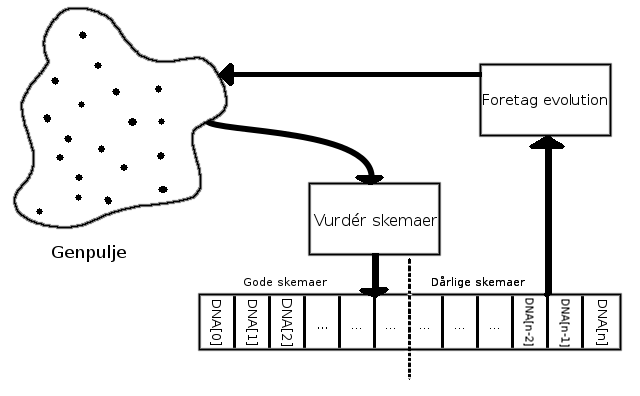
\includegraphics[width=0.8\textwidth]{loesningsdiagram.png}
	\caption{Løsningsdiagram til vores program}
	\label{fig:loesningsdiagram}
\end{figure}